%----------------------------------------------------------------
%
%  File    :  implementation.tex
%
%  Authors :  David Lechner, FH Campus Wien, Austria
%
%  Created :  10 Oct 2019
%
%  Changed :  10 Oct 2019
%
%----------------------------------------------------------------


\chapter{Umsetzung}
\label{chap:back}

Dieses Kapitel geht auf die konkrete Umsetzung des Systems ein. Anfangs werden die zur Verfügung stehenden Daten beschrieben und wie diese für \textit{Machine Learning} vorverarbeitet werden. Danach werden die eingesetzten ML-\textit{Model} erklärt und die Optimierung dieser gezeigt. Den Abschluss bildet die Integration in ein Fahrzeug.

\section{CAN-Daten}
\label{sec:data_description}

Bei den Daten, welche für die Masterarbeit vorliegen, handelt es sich um CAN-Nachrichten, aufgenommen in zehn Fahrzeugen (VW Golf 7, keine näheren Informationen) während dem Fahren. Dabei ist sichergestellt, dass jeweils nur eine Person hinter dem Lenkrad gesessen ist. Für die Aufzeichnung wurde ein Boardcomputer mit Internetkonnektivität (\textit{ALEN}, siehe \ref{sec:alen}) im Fahrerraum verwendet. Das \textit{Embedded-Device} ist über zwei CAN-Bus Schnittstellen mit der Fahrwerks-Linie (F-CAN) und der Fahrzeugelektrik-Linie (K-CAN) verbunden und kann somit alle Nachrichten in fast-echtzeit vom Bus mitlesen. Dabei ist aber sichergestellt, dass es nicht möglich ist, auch Nachrichten senden zu können, da dies bei einer Fehlfunktion zu einem Unfall führen und Insaßen gefährden könnte. Die Nachrichten werden nach dem Empfangen mit einem synchronisierten Zeitstempel, aufgelöst in Nanosekunden, versehen und in eine MDF Datei mit den Metadaten von der entsprechenden DBC-Datenbank gespeichert. Eine Datei enthält jeweils Messdaten über eine Dauer von einer Minute. Danach wurde die Datei temporär auf einer Festplatte gespeichert und auf einem File-Server über eine LTE-Funkverbindung hochgeladen. Um sie über alle Fahrzeuge hinweg eindeutig zuordnen zu können, wurde eine Fahrzeugidentifikationsnummer dem Dateinamen angehängt.

In einer Datei sind 46 verschiedene Signale der beiden CAN-Busse enthalten. Tablle \ref{tab:can_signals} listet die meisten davon. Jene, die sich vorrausichtlich nicht für die Analyse eignen, wie z.B. die innen Temperatur oder der Status des Standlichts, sind ausgenommen. Für die komplette Liste siehe Anhang. Pro Datei sind durchschnittlich 100000 Messwerte vorhanden, daraus ergeben sich bei einer Anzahl von 10359 Dateien über eine Milliarde Messpunkte. Die folgende Liste gibt einen Einblick über die vorhandenen Daten.
% TODO: Anhang mit kompletter Liste

\begin{itemize}
  \item Anzahl Fahrer: 10
  \item Datengröße (MDF): 3,7 GB
  \item $\diameter$ Fahrtenanzahl: 1
  \item Fahrtenanzahl insgesamt: 7
  \item $\diameter$ Fahrtzeit pro Fahrer pro Fahrt: 13
  \item $\diameter$ Fahrtzeit pro Fahrer: 14
  \item Fahrtzeit insgesamt: 87
  \item $\diameter$ Gefahrene Kilometer: 14
  \item Gefahrene Kilometer insgesamt: 84
  \item Zeitraum: 12.09.2019 - 13.08.2019
\end{itemize}

\begin{table*}[htbp]
	\centering
		\begin{tabular}{|l|l|l|l|l|}
		\hline
		\rowcolor[gray]{0.9}
		Signalname & CAN-Bus & Beschreibung & Einheit & Wertbeschr. \\
		\hline
    LWI\_Lenkradwinkel & F-CAN & Lenkradwinkel & Grad & - \\
    LWI\_VZ\_Lenkradwindel & F-CAN & \shortstack{Vorzeichen von \\ Lenkradwinkel} & Boolean & \shortstack{0: Positiv \\ 1: Negativ} \\
    ESP\_Fahrer\_bremst & F-CAN & Bremspedal betätigt & Boolean & \shortstack{0: nicht betätigt \\ 1: betätigt} \\
    ESP\_Bremsdruck & F-CAN & Bremsdruck & Bar & - \\
    MO\_Fahrpedalrohwert\_01 & F-CAN & Fahrpedalposition & - & - \\
    MO\_Kuppl\_schalter & F-CAN & Kupplung betätigt & Boolean & \shortstack{0: nicht betätigt \\ 1: betätigt} \\
    MO\_Drehzahl\_01 & F-CAN & Motordrehzahl & rpm & - \\
    KBI\_Tankfuellstand\_Prozent & F-CAN & Tankfüllstand & \% & - \\
    KBI\_Kilometerstand & F-CAN & Kilometerstand & km & - \\
    MO\_Gangposition & F-CAN & Gangposition & - & \shortstack{1: 1. Gang oder \\ Rückwärtsgang \\ 2-6: 2. - 6. Gang} \\
    ESP\_VL\_Radgeschw\_02 & F-CAN & \shortstack{Geschwindigkeit \\ Rad links vorne} & km/h & - \\
    ESP\_VR\_Radgeschw\_02 & F-CAN & \shortstack{Geschwindigkeit \\ Rad rechts vornen} & km/h & - \\
    ESP\_HL\_Radgeschw\_02 & F-CAN & \shortstack{Geschwindigkeit \\ Rad links hinten} & km/h & - \\
    ESP\_HR\_Radgeschw\_02 & F-CAN & \shortstack{Geschwindigkeit \\ Rad rechts hinten} & km/h & - \\
    ESP\_v\_Signal & F-CAN & \shortstack{Durchschnittliche \\ Radgeschwindigkeit} & km/h & - \\
    ESP\_HL\_Fahrtrichtung & F-CAN & \shortstack{Fahrtrichtung \\ Rad links hinten} & - & \multirow{2}{*}{\shortstack{0: Vorwärts \\ 1: Rückwärts}} \\
    ESP\_HL\_Fahrtrichtung & F-CAN & \shortstack{Fahrtrichtung \\ Rad links hinten} & - & \\
    ESP\_Laengsbeschl & F-CAN & Längsbeschleunigung & m/s\textsuperscript{2} & - \\
    ESP\_Querbeschleinigung & F-CAN & Querbeschleunigung & m/s\textsuperscript{2} & - \\
    ESP\_Gierrate & F-CAN & Gierrate & \shortstack{Grad pro \\ Sekunde} & - \\
    ESP\_VZ\_Gierrate & F-CAN & \shortstack{Vorzeichen \\ von Gierrate} & Boolean & \shortstack{0: Positiv \\ 1: Negativ} \\
    Wischer\_vorne\_aktiv & K-CAN & Wischer vorne aktiv & Boolean & \multirow{3}{*}{\shortstack{0: nicht aktiv \\ 1: aktiv}} \\
    BH\_Blinker\_li & K-CAN & Blinker links aktiv & Boolean & \\
    BH\_Blinker\_re & K-CAN & Blinker rechts aktiv & Boolean & \\
		\hline
		\end{tabular}
	\caption{Signalbeschreibung}
	\label{tab:can_signals}
\end{table*}

Je nach Steuergerät und Nachrichtentyp ist die Signalhäufigkeit unterschiedlich. Zum Beispiel sendet das Lenkrad- und Motorsteuergerät mit der gleichen Frequenz – nämlich 100-mal in der Sekunde. Andere jedoch, wie das Getriebesteuergerät, nur mit einer Frequenz von 10 Hz. Abbildung \ref{fig:signal_freq} zeigt Häufigkeit einiger Signale.

\begin{figure}[htbp]
	\centering
		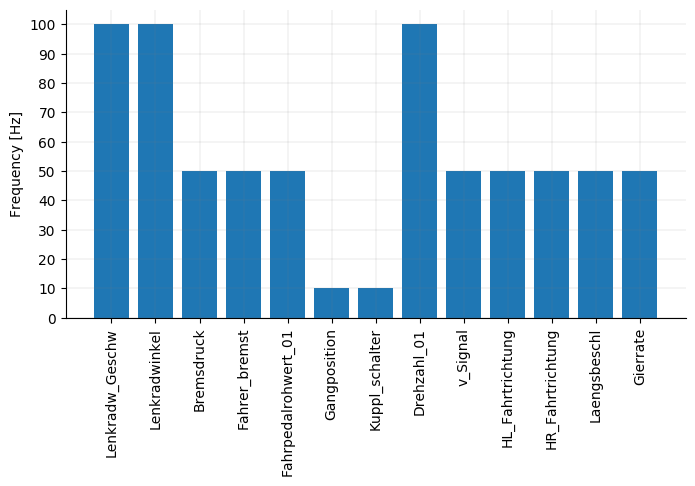
\includegraphics[width=\textwidth]{images/signal_frequences.png}
	\caption{Signalhäufigkeiten (Quelle: Author)}
	\label{fig:signal_freq}
\end{figure}

\section{Trainingsdaten}
\label{sec:train_data}

Relevante

Data transformation

Feature extraction

\section{Machine Learning Model}
\label{sec:ml_implementation}

Wieso supervised und nicht zb unsupervised? daten sind bereits markiert, kein zeitaufwand notwendig, bessere genauigkeit. trotzdem probieren! ML Model beschreiben, Code snippets

\subsection{Optimierung}
\label{sec:ml_optimization}

Hyper parametering, trade of performance - accuracy

\section{Integration in Auto}
\label{sec:car_integration}

ML auf ALEN Box

\subsection{Automotive Linux Edge Node (ALEN)}
\label{sec:alen}